We discuss the effect of strong many-body interactions in a Dirac semimetal in three dimensions. Before we do so, it is worth stepping back and reviewing the two dimensional case in order to illustrate the issue and idea that will be considered and generalized in three dimensions. The massless Dirac fermion with $H=\hbar v(k_xs_y-k_ys_x)$ that appears on the surface of a topological insulator~\cite{HasanKane10,QiZhangreview11,HasanMoore11,RMP} is protected by time reversal (TR) and charge $U(1)$ symmetries and is anomalous. This means that there is no single-body energy gap opening mass term that preserves the symmetries, and there is no single-body fermionic lattice model in two dimensions that supports a massless Dirac fermion without breaking the symmetries. Neither of these statements hold true in the many-body setting. The surface Dirac fermion can acquire a time reversal and charge $U(1)$ preserving many-body interacting mass.~\cite{WangPotterSenthilgapTI13,ChenFidkowskiVishwanath14,MetlitskiKaneFisher13b,BondersonNayakQi13} Consequently, this also enables a massless symmetry preserving Dirac fermion in a pure 2D system without holographically relying on a semi-infinite 3D topological bulk. For instance, one can take a quasi-2D topological insulator slab with finite thickness and remove the Dirac fermion on one of the two surfaces by introducing an interacting mass gap. This leaves a single massless Dirac fermion on the opposite surface without breaking symmetries.

A massless Dirac fermion in three dimensional semimetallic materials can be protected in the single-body picture by screw rotation, time reversal and charge $U(1)$ symmetries (see reviews Ref.~\onlinecite{Ashvin_Weyl_review,RMP,ArmitageMeleVishwanath16} and section~\ref{sec:DiracSemimetal}). From a theory point of view, it can be supported on the 3D boundary of a 4D weak topological insulator, where the two Weyl fermions are located at distinct time reversal invariant momenta (recall figure~\ref{fig:Weylspectrum} and section~\ref{sec:holproj4D} for the antiferromagnetic case). In this case, the massless fermions are protected by translation, time reversal and charge $U(1)$ symmetries. In this section, we address the following issues. (1) We show by explicitly constructing an exactly solvable coupled wire model that the 3D Dirac fermion can acquire a many-body interacting mass while preserving all symmetries. (2) We show in principle that an antiferromagnetic time reversal (AFTR) symmetric massless 3D Dirac system with two Weyl fermions separated in momentum space can be enabled by many-body interactions without holographically relying on a higher dimensional topological bulk.

We begin with the Dirac semimetallic coupled wire model in figure~\ref{fig:Weylspectrum} and \eqref{WeylTBHam}.  


\subsubsection{Symmetry preserving massive interacting model}\label{sec:interactionmodels}

We begin with the 3D array of chiral Dirac strings in figure~\ref{fig:vortexlattice}. In section~\ref{sec:DiracSemimetal}, we showed that the single-body coupled wire model \eqref{WeylTBHam} described a Dirac semimetal with two Weyl fermions (see figure~\ref{fig:Weylspectrum}). The system had emergent antiferromagnetic time reversal (AFTR) symmetries $\mathcal{T}_{11}$ and $\mathcal{T}_{\bar{1}1}$ along the diagonal and off-diagonal axes (see \eqref{WeylTBT11}). Together they generate an emergent lattice translation symmetry with a 2-wire unit cell, and separate the two Weyl points in the Brillouin zone. The symmetries are lowered beyond the effective model when the microscopic high-energy degrees of freedom are included. For example, the mass function \eqref{Jacobielliptic} that supports the Dirac vortex string lattice has a 4-wire periodic unit cell and only preserves one of the \AFTR symmetries $\mathcal{T}_{11}$ (see \eqref{massT11}). With the lowered translation symmetry, the two Weyl points now coincide at the same momentum. Inter-species (or inter-valley) mixing is forbidden by the remaining \AFTR symmetry and a (screw) twofold rotation symmetry $C_2$ about $z$ (see \eqref{WeylTBC2} and \eqref{massC2}). Previously in section~\ref{sec:brokensymmetry}, we introduced symmetry breaking wire dimerizations in \eqref{DiracTBHam} that led to a massive Dirac insulator. In this section, we construct many-body gapping interactions that preserves the two \AFTR symmetries $\mathcal{T}_{11}$ and $\mathcal{T}_{\bar{1}1}$, the $C_2$ symmetry, as well as charge $U(1)$ conservation. 

\begin{figure}[htbp]
\centering
(a)\includegraphics[width=0.25\textwidth]{gappinginteraction1}
(b)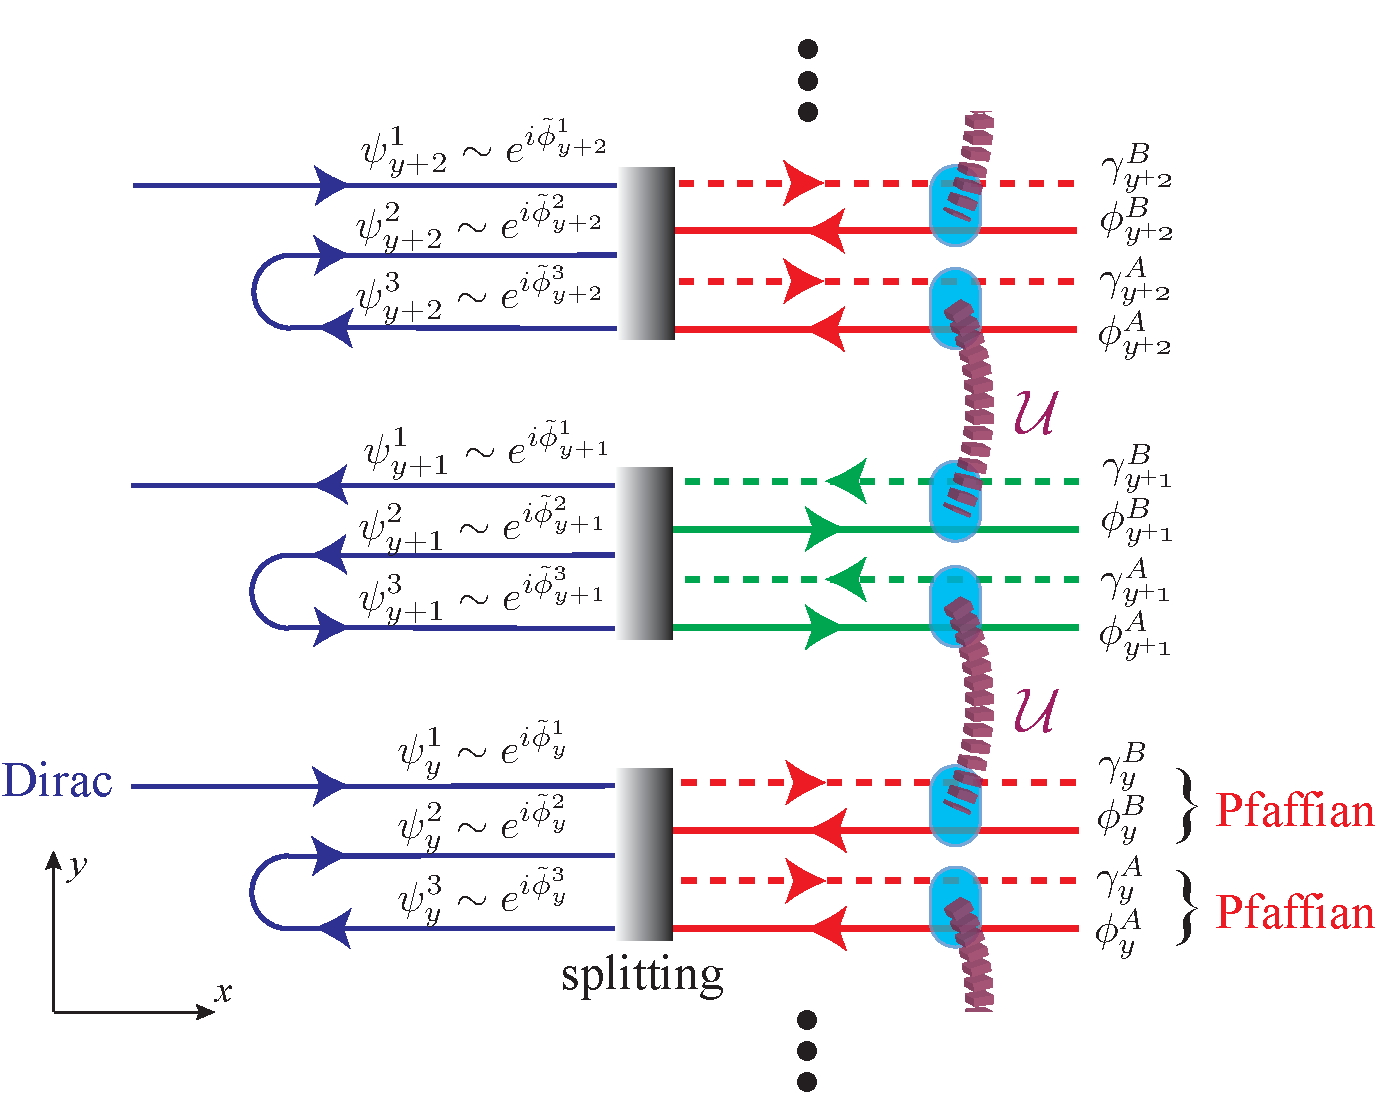
\includegraphics[width=0.45\textwidth]{gappinginteraction2}
\caption{Symmetry preserving many-body gapping interaction. (a) Each {\color{red}$\boldsymbol\times$}/{\color{green}$\bullet$} represents a chiral Pfaffian channel into/out-of paper. Purple dashed line represents many-body gapping interaction $\mathcal{U}$ in \eqref{mbdint}. (b) Coupled wire model on a single layer along the diagonal axis.}\label{fig:gappinginteraction}
\end{figure}

The many-body gapping scheme is summarized in figure~\ref{fig:gappinginteraction}. From the previous subsection, we saw that each chiral Dirac channel can be decomposed into a pair of independent Pfaffian channels. They can then be backscattered in opposite directions to neighboring wires. Figure~\ref{fig:gappinginteraction}(a) shows a particular dimerization pattern of the Pfaffian channels that preserves the symmetries. In this case, the many-body backscattering interaction $\mathcal{U}$ is directed along the diagonal axis. In the limit when $\mathcal{U}$ is much stronger than the single-body electron tunneling in the previous semimetallic model \eqref{WeylTBHam}, the system decomposes into decoupled diagonal layers and it suffices to consider the interaction on a single layer. For convenience, we here change our spatial coordinates so that the diagonal axis is now labeled by $y$ and the wires now propagate along $x$.

Focusing on a single diagonal layer, the system in the non-interacting limit first consists of a 2D array of chiral Dirac strings with alternating propagating directions (see the left side of figure~\ref{fig:gappinginteraction}(b)). We notice that this is identical to the starting point of the coupled wire construction of the topological insulator Dirac surface state considered by Mross, Essin and Alicea in Ref.~\onlinecite{MrossEssinAlicea15}. For instance, the alternating Dirac channels there were supported between magnetic strips with alternating orientations on the topological insulator surface, and an uniform nearest-channel electron tunneling recovered the massless 2D Dirac spectrum protected by the \AFTR symmetry. They then proceeded to propose symmetry preserving many-body gapping interactions facilitated by adding 2D fractional quantum hall strips between the channels. While this reconstruction trick can be applied on the 2D surface of a topological insulator, it is not feasible in our 3D situation and would require drastic modification of the bulk semimetal. Instead, here we propose an alternative gapping scheme that does not involve additional topological phases. In other words, we are going to construct a 3D gapped and layered topological phase solely from interacting electronic Dirac wires.

First, in order to implement the splitting described in the previous subsection, we assume each Dirac string consists of two Dirac channels going in one direction and a third Dirac channel going the opposite direction (see the left side of figure~\ref{fig:gappinginteraction}(b)). We denote the electronic Dirac fermions on the $y^{\mathrm{th}}$ wire by $\boldsymbol\psi_y=(\psi_y^1,\psi_y^2,\psi_y^3)$ and bosonize \begin{align}\psi_y^{1,2}(x)\sim e^{i\tilde\phi^{1,2}_y(x)},\quad\psi_y^3(x)\sim e^{-i\tilde\phi^3_y(x)}.\label{bosondef}\end{align} The sliding Luttinger liquid\cite{OHernLubenskyToner99,EmeryFradkinKivelsonLubensky00,VishwanathCarpentier01,SondhiYang01,MukhopadhyayKaneLubensky01} Lagrangian density is \begin{align}\mathcal{L}_{\mathrm{layer}}=\sum_{y=-\infty}^\infty\frac{(-1)^y\tilde{K}_{jk}}{2\pi}\partial_t\tilde\phi_y^j\partial_x\tilde\phi_y^k+\tilde{V}_{jk}\partial_x\tilde\phi_y^j\partial_x\tilde\phi_y^k\label{Llayer}\end{align} where $\tilde{K}=(\tilde{K}_{jk})_{3\times3}=\mathrm{diag}(1,1,-1)$, $\tilde{V}$ is some non-universal velocity matrix, and repeating species indices $j,k$ are summed over. The boson operators obey the equal-time commutation relation (\hypertarget{ETCR}{ETCR}) \begin{align}&\left[\tilde\phi_y^j(x),\tilde\phi_{y'}^{j'}(x')\right]=c^{jj'}_{yy'}(x-x')\nonumber\\=&i\pi(-1)^y\delta_{yy'}\tilde{K}^{jj'}\mathrm{sgn}(x'-x)\label{ETcomm0}\\&+i\pi(-1)^y\delta_{yy'}S^{jj'}\nonumber\\&+i\pi(-1)^{\mathrm{max}\{y,y'\}}\mathrm{sgn}(y-y')\Sigma^{jj'}\sigma_z^{y-y'+1}\nonumber\end{align}
%\begin{align}\left[\tilde\phi_y^j(x),\tilde\phi_{y'}^{j'}(x')\right]=&i\pi(-1)^{\mathrm{max}\{y,y'\}}\Big[\delta_{yy'}\tilde{K}^{jj'}\mathrm{sgn}(x'-x)\nonumber\\&+\delta_{yy'}\mathrm{sgn}(j-j')+\mathrm{sgn}(y-y')\Big]\label{ETcomm0}\end{align} 
where $\mathrm{sgn}(s)=s/|s|=\pm1$ for $s\neq0$ and $\mathrm{sgn}(0)=0$, \begin{align}S=\left(\begin{smallmatrix}0&1&-1\\-1&0&1\\1&-1&0\end{smallmatrix}\right),\quad\Sigma=\left(\begin{smallmatrix}1&1&-1\\1&1&-1\\-1&-1&1\end{smallmatrix}\right),\label{Kleinfactors}\end{align} and $\sigma_z=\pm1$. The introduction of the specific Klein factors $S^{jj'}$, $\Sigma^{jj'}$ and the undetermined sign $\sigma_z$ are necessary for the correct representations of the $\mathcal{T}_{11}$ and $\mathcal{C}_2$ symmetries in the bosonization setting, and these choices will be justified below. The first line of \eqref{ETcomm0} is equivalent to the commutation relation between conjugate fields \begin{align}\left[\tilde\phi_y^j(x),\partial_{x'}\tilde\phi_{y'}^{j'}(x')\right]=2\pi i(-1)^y\delta_{yy'}\tilde{K}^{jj'}\delta(x-x')\label{ETcomm00}\end{align} which is set by the ``$p\dot{q}$" term in $\mathcal{L}_{\mathrm{layer}}$. The alternating signs $(-1)^y$ in \eqref{ETcomm00} and \eqref{Llayer} changes the propagating directions from wire to wire. The second and third line of \eqref{ETcomm0} guarantee the correct anticommutation relations $\{e^{\pm i\tilde\phi^j_y},e^{\pm i\tilde\phi^{j'}_{y'}}\}=0$ between Dirac fermions along distinct channels $j\neq j'$ or distinct wires $y\neq y'$. The reason the $\tilde{C}_2$ matrix is defined in this form will become clear in the fractional basis discussed later in \eqref{bosonC2Pf}.

The anti-unitary \AFTR symmetry along the diagonal $\mathcal{T}_{11}$ direction transforms the bosons according to \begin{align}\mathcal{T}_{11}\tilde\phi^j_y\mathcal{T}_{11}^{-1}=-\tilde\phi^j_{y+1}+\frac{1+(-1)^y}{2}\tilde{K}^{jj}\pi.\label{bosonTR11}\end{align} The unitary $\mathcal{C}_2$ rotation takes \begin{gather}\mathcal{C}_2\tilde\phi^j_y\mathcal{C}_2^{-1}=\left(\tilde{C}_2\right)^j_{j'}\tilde\phi^{j'}_{-y}+(-1)^yv^j\frac{\pi}{2},\label{bosonC2}\\\tilde{C}_2=\left(\begin{smallmatrix}1&2&2\\2&1&2\\-2&-2&-3\end{smallmatrix}\right),\quad{\bf v}=\left(\begin{smallmatrix}v^1\\v^2\\v^3\end{smallmatrix}\right)=\left(\begin{smallmatrix}3\\-3\\1\end{smallmatrix}\right).\nonumber\end{gather} Moreover, we choose the representation so that the sign $\sigma_z$ in the equal time commutation relations \eqref{ETcomm0} is preserved by the \AFTR operator but is flipped by the $C_2$ symmetry, \begin{align}\mathcal{T}_{11}\sigma_z\mathcal{T}_{11}^{-1}=\sigma_z,\quad\mathcal{C}_2\sigma_z\mathcal{C}_2^{-1}=-\sigma_z.\end{align} 

The equal time commutation relations \eqref{ETcomm0} is consistent with the \AFTR symmetry. This means that evaluating $\mathcal{T}_{11}\left[\tilde\phi_y^j(x),\tilde\phi_{y'}^{j'}(x')\right]\mathcal{T}_{11}^{-1}$ by taking the \AFTR operator inside the commutator \begin{align}&\left[\mathcal{T}_{11}\tilde\phi_y^j(x)\mathcal{T}_{11}^{-1},\mathcal{T}_{11}\tilde\phi_{y'}^{j'}(x')\mathcal{T}_{11}^{-1}\right]\nonumber\\&=\left[\tilde\phi_{y+1}^j(x),\tilde\phi_{y'+1}^{j'}(x')\right]=c^{jj'}_{y+1,y'+1}(x-x')\end{align} yields the same outcome as taking the time reversal of the purely imaginary scalar \begin{align}\mathcal{T}_{11}c^{jj'}_{yy'}(x-x')\mathcal{T}_{11}^{-1}=-c^{jj'}_{yy'}(x-x').\end{align} The equal time commutation relations \eqref{ETcomm0} is also consistent with the $\mathcal{C}_2$ symmetry \begin{align}(\tilde{C}_2)^{j_1}_{j'_1}c^{j'_1j'_2}_{-y_1,-y_2}(x_1-x_2)(\tilde{C}_2)^{j_2}_{j'_2}=\mathcal{C}_2c^{j_1j_2}_{y_1y_2}(x_1-x_2)\mathcal{C}_2^{-1}.\label{ETcommC2consistent}\end{align} This is because the Klein factors \eqref{Kleinfactors} are $C_2$ symmetric \begin{align}\tilde{C}_2S\tilde{C}_2^T=S,\quad\tilde{C}_2\Sigma\tilde{C}_2^T=\Sigma.\end{align} Notice that the undetermined sign $\sigma_z$, which is odd under $\mathcal{C}_2$, in \eqref{ETcomm0} is essential for the equal time commutation relations to be consistent with $C_2$.

The last term in the \AFTR operation \eqref{bosonTR11} makes sure \begin{align}\mathcal{T}_{11}^2\tilde\phi_y^j(x)\mathcal{T}_{11}^{-2}=\tilde\phi_{y+2}^j+(-1)^y\tilde{K}^{jj}\pi,\end{align} which is necessary for $\mathcal{T}^2_{11}=(-1)^F\mathrm{translation}(2{\bf e}_y)$. Here the fermion parity operator is $(-1)^F=e^{i\pi\sum_{yj}N_y^j}$, where \begin{align}N_y^j=\int\frac{dx}{2\pi}\partial_x\tilde\phi_y^j(x)\label{numop}\end{align} is the number operator. The vector ${\bf v}$ in the $\mathcal{C}_2$ operation \eqref{bosonC2} satisfies $(\delta^j_{j'}+(\tilde{C}_2)^j_{j'})v^{j'}/2=\tilde{K}^{jj}$, and consequently \begin{align}\mathcal{C}_{2}^2\tilde\phi_y^j(x)\mathcal{C}_{2}^{-2}=\tilde\phi_y^j+(-1)^y\tilde{K}^{jj}\pi,\end{align} which is consistent with $\mathcal{C}_2^2=(-1)^F$. Lastly, it is straightforward to check that the symmetry representations \eqref{bosonTR11} and \eqref{bosonC2} are compatible with the algebraic relation \eqref{C2Trelation}, i.e. \begin{align}&\mathcal{C}_2\mathcal{T}_{11}\tilde\phi^j_y\mathcal{T}_{11}^{-1}\mathcal{C}_2^{-1}\\&=(-1)^F\mathcal{T}_{11}^{-1}\mathcal{C}_2\tilde\phi^j_y\mathcal{C}_2^{-1}\mathcal{T}_{11}(-1)^{-F}.\nonumber\end{align}

%The, at first sight, obscured expression of the $3\times3$ rotation matrix $C_2$ in \eqref{bosonC2} actually takes a much simply form under the fractional basis transformation considered in the previous subsection~\ref{sec:gluing}. We defer this simplification a bit later, but at this point, we notice that the Klein fators $S$ and $\Sigma$ in the \ETCR \eqref{ETcomm0} are chosen to be consistent with the $C_2$ symmetry, \begin{align}C_2SC_2^T=S,\quad C_2\Sigma C_2^T=\Sigma.\end{align} 

Following the splitting scheme summarized in figure~\ref{fig:fractionalization}, we again define a fractional basis transformation (c.f.~\eqref{fracbasistrans0}) \begin{align}\begin{pmatrix}\phi^\rho_y\\\phi^{\sigma1}_y\\\phi^{\sigma2}_y\end{pmatrix}=\left(\begin{array}{*{20}c}1&1&1\\1&-1/2&1/2\\1&1/2&3/2\end{array}\right)\left(\begin{array}{*{20}c}\tilde\phi^1_y\\\tilde\phi^2_y\\\tilde\phi^3_y\end{array}\right)\label{fracbasistrans}\end{align} for each wire, so that $\psi^\rho_y\sim e^{i\phi^\rho_y}$ is a Dirac fermion carrying electric charge $e$, $d^{\sigma1}_y\sim e^{i\phi^{\sigma1}_y}$ ($d^{\sigma2}_y\sim e^{i\phi^{\sigma2}_y}$) is an electrically neutral Dirac fermion propagating in the same (resp.~opposite) direction as $\psi^\rho_y$.

For convenience, sometimes we combine the transformed bosonized variables into $\boldsymbol\phi_y=(\phi^1_y,\phi^2_y,\phi^3_y)=(\phi^A_y,\phi^B_y,\phi^{\sigma2}_y)$, which is related to the original local ones in \eqref{Llayer} by $\phi^J_y=G^J_j\tilde\phi^j_y$ where \begin{align}G=\begin{pmatrix}1/2&1/8&3/8\\0&3/8&1/8\\1&1/2&3/2\end{pmatrix}.\end{align} The \AFTR symmetry operation \eqref{bosonTR11} becomes \begin{align}\mathcal{T}_{11}\phi^I_y\mathcal{T}_{11}^{-1}=-\phi^I_{y+1}+\frac{1+(-1)^y}{2}\pi\kappa^I\label{bosonTR11Pf}
%\mathcal{T}_{11}\phi^{A/B}_y\mathcal{T}_{11}^{-1}&=-\phi^{A/B}_{y+1}+\frac{1+(-1)^y}{2}\pi,\nonumber\\\mathcal{T}_{11}\phi^{\sigma 2}_y\mathcal{T}_{11}^{-1}&=-\phi^{\sigma 2}_{y+1}.
\end{align} where $\kappa^I=G^I_j\tilde{K}^{jj}$ which is $1/4$ for $I=1,2$ and $0$ for $I=3$. The $C_2$ transformation \eqref{bosonC2} becomes \begin{gather}\mathcal{C}_2\phi^I_y\mathcal{C}_2^{-1}=\left(C_2\right)^I_J\phi^J_{-y}+(-1)^yG^I_jv^j\frac{\pi}{2},\label{bosonC2Pf}\\C_2=G\tilde{C}_2G^{-1}=\left(\begin{smallmatrix}0&1&0\\1&0&0\\0&0&-1\end{smallmatrix}\right),\quad G{\bf v}=\left(\begin{smallmatrix}3/2\\-1\\3\end{smallmatrix}\right).\nonumber\end{gather} The $3\times3$ $C_2$ matrix takes a much simpler form here using the fractional basis than in \eqref{bosonC2}. In fact, the original $\tilde{C}_2$ matrix in the local basis in \eqref{bosonC2} was defined so that $C_2=G\tilde{C}_2G^{-1}$ would act according to \eqref{bosonC2Pf}. Roughly speaking, ignoring the constant phases $G{\bf v}$, the $C_2$ symmetry switches $\phi^A_y\leftrightarrow\phi^B_{-y}$ and sends $\phi^{\sigma2}_y\to-\phi^{\sigma2}_{-y}$.

Next, we combine these co-propagating pair of fermions to form two $SU(2)_1$ current algebras (c.f.~\eqref{SU2current} and \eqref{SU2algebra}) \begin{align}&J_3^{A/B}(y,w)=i2\sqrt{2}\partial_w\phi^{A/B}_y(w)\nonumber\\&J_\pm^{A/B}(y,w)=e^{\pm i4\phi^{A/B}_y(w)}%\\&4\phi^A_y(w)=\phi^\rho_y(w)+\phi^{\sigma1}_y(w),\quad 4\phi^B_y(w)=\phi^\rho_y(w)-\phi^{\sigma1}_y(w)\nonumber
\end{align} where $w\sim\tau+(-1)^yx$ is the complex spacetime parameter. As a reminder, the charge $\pm e$ bosons $J^{A/B}_\pm$ are non-electronic fractional operators, although they carry non-fractional statistics.

The remaining counter-propagating neutral Dirac fermion can be decomposed into real and imaginary components \begin{align}d_y^{\sigma}(w)\sim\cos\phi^{\sigma2}_y(w)+i\sin\phi^{\sigma2}_y(w).\end{align} Majorana fermions can be constructed by multiplying these components with ``Jordan-Wigner" string \begin{align}\gamma^A_y&\sim\cos\phi^{\sigma2}_y\prod_{y'>y}(-1)^{N_{y'}^2+N_{y'}^3},\nonumber\\\gamma^B_y&\sim\sin\phi^{\sigma2}_y\prod_{y'>y}(-1)^{N_{y'}^2+N_{y'}^3},\label{MFdef}\end{align} where $N^j_y$ are the number operators defined in \eqref{numop}, so that they obey mutual fermionic statistics $\{\gamma^\lambda_y(x),\gamma^{\lambda'}_{y'}(x')\}=\delta^{\lambda\lambda'}\delta_{yy'}\delta(x-x')$, for $\lambda,\lambda'=A,B$. Similar to the charge  $\pm e$ bosons $J^{A/B}_\pm$, the electrically neutral Dirac fermion $d_y^\sigma$ and consequently the Majorana fermions $\gamma^{A/B}_y$ are also non-electronic fractional operators. This $AB$-decomposition splits each Dirac wire into a pair of decoupled Pfaffian sectors (see figure~\ref{fig:gappinginteraction}(b)).

Before we move on to the symmetric interaction, some further elaborations are needed for the number operators $N_y^j$ and their corresponding fermion parity operators $e^{i\pi N_y^j}$. In our construction, the counter-propagating pair of channels with $j=2,3$ are appended to the original one with $j=1$ to make the Pfaffian fractionalization feasible. We choose the Hilbert space so that the two additional fermion parity operators agree, $e^{i\pi N_y^2}=e^{i\pi N_y^3}$. However, we allow fluctuations to the combined parity $e^{i\pi(N_y^2+N_y^3)}$ and only require it squares to the identity, $e^{2\pi i(N_y^2+N_y^3)}=1$. In other words, $e^{i\pi(N_y^2+N_y^3)}=e^{-i\pi(N_y^2+N_y^3)}$ and it does not matter which one we take as $(-1)^{N_y^2+N_y^3}$ in the ``Jordan-Wigner" string in \eqref{MFdef}. This convention will also be useful later in seeing that the many-body interaction is exactly solvable and symmetry preserving. Extra care is sometimes required. For example, unlike the original Dirac channel where the parity is simply $(-1)^{N_y^1}=e^{\pm i\pi N_y^1}$ because $e^{2\pi iN_y^1}=1$, the individual parity operators $(-1)^{N_y^{2,3}}$ of these additional channels are not well-defined because $e^{2\pi iN_y^{2,3}}\neq1$, i.e.~$e^{i\pi N_y^{2,3}}\neq e^{-i\pi N_y^{2,3}}$. Also, although $e^{2\pi i(N_y^2+N_y^3)}=1$, one cannot in general modify a boson angle parameter simply by $\Theta\to\Theta+2\pi i(N_y^2+N_y^3)$ because $\Theta$ and the number operators may not commute. For instance, using the Baker-Campbell-Hausdorff formula and the equal time commutation relations \eqref{ETcomm0}, $e^{i4\phi^{A/B}}$ and $e^{i4\phi^{A/B}+2\pi i(N_y^2+N_y^3)}$ are off by a minus sign.

The Pfaffian fractionalization is stablized by the inter-wire many-body backscattering interaction (see figure~\ref{fig:gappinginteraction}(b)) \begin{align}\mathcal{U}&=-u\sum_{y=-\infty}^\infty\cos\phi^{\sigma2}_{y+1}\sin\phi^{\sigma2}_y\cos\left(4\phi^A_{y+1}-4\phi^B_y\right)\nonumber\\
&=-u\sum_{y=-\infty}^\infty(-1)^yi\gamma^A_{y+1}\gamma^B_y\cos\left(\Theta_{y+1/2}\right),\label{mbdint}\end{align} for $\Theta_{y+1/2}(x)=4\phi^A_{y+1}(x)-4\phi^B_y(x)+\pi(N_{y+1}^2+N_{y+1}^3)$. Previously in \eqref{psi4def1}, we saw that the combinations $\psi_4^A\sim e^{i4\phi^A}\gamma^A$ and $\psi_4^B\sim e^{i4\phi^B}\gamma^B$ can be decomposed into products of electron operators. Similarly, each interaction in the first line of \eqref{mbdint} can be decomposed into products in the form of $e^{\pm i(\phi^{\sigma2}_{y+1}\pm4\phi^A_{y+1})}e^{\pm i(\phi^{\sigma2}_y\pm4\phi^B_y)}$ (with some scalar $U(1)$ coefficient), where the exponents $\phi^{\sigma2}\pm4\phi^{A/B}$ are linear integral combinations of $\tilde\phi^j$. Thus, the interaction can be re-written in terms of backscatterings of local electronic operators. However, we will omit the electronic expression as \eqref{mbdint} is more useful in discussing ground state and symmetries. 

$\mathcal{U}$ describes a symmetry-preserving exactly solvable model. Using the equal time commutation relations \eqref{ETcomm0} it is straightforward to check that the (normal ordered) order parameters \begin{align}\mathcal{O}_{y+1/2}^F(x)=i\gamma^A_{y+1}(x)\gamma^B_y(x),\quad\mathcal{O}_{y+1/2}^\Theta(x)=e^{i\Theta_{y+1/2}(x)}\label{orderparameters}\end{align} mutually commute, i.e. $\left[\mathcal{O}_{y+1/2}^{F/\Theta}(x),\mathcal{O}_{y'+1/2}^{F/\Theta}(x')\right]=0$. Therefore, the model is exactly solvable, and its ground states are characterized by the ground state expectation values of the order parameters \begin{align}l_0\langle\mathcal{O}_{y+1/2}^F\rangle=(-1)^y\langle\mathcal{O}_{y+1/2}^\Theta\rangle=\pm1\end{align} so that the interacting energy $\langle\mathcal{U}\rangle$ is minimized, where $l_0$ is some non-universal microscopic length scale. Pinning the ground state expectation values $\langle\Theta_{y+1/2}\rangle=n_{y+1/2}\pi$, for $n_{y+1/2}\in\mathbb{Z}$, gaps all degrees of freedom in the charged $U(1)_4^{A/B}=SU(2)_1^{A/B}$ sector. The remaining neutral fermions are gapped by the decoupled Majorana backscattering \begin{align}\delta\mathcal{H}_{\mathrm{Majorana}}=u\sum_{y=-\infty}^\infty(-1)^yi\langle\mathcal{O}^\Theta_{y+1/2}\rangle\gamma^A_{y+1}\gamma^B_y.\label{MajHam}\end{align} It is worth noting that a $\pi$-kink excitation of $\langle\Theta_{y+1/2}\rangle$ flips the Majorana mass in \eqref{MajHam} and therefore bounds a zero energy Majorana bound state~\cite{Kitaevchain}. A $\pi$-kink at $x_0$ can be created by the vertex operators $e^{\pm i\phi^A_{y+1}(x_0)}$ or $e^{\pm i\phi^B_y(x_0)}$ which carry $\pm1/4$ of an electric charge. (Recall the bosonic vertices $e^{i4\phi^{A/B}_y}$ carry charge $e$.) This $e/4$ excitation therefore corresponds to the Ising anyon in the Pfaffian fractional quantum hall state.

From the \AFTR symmetry action \eqref{bosonTR11Pf}, one can show that the Majorana fermions \eqref{MFdef} transform according to \begin{align}\mathcal{T}_{11}\gamma^A_y\mathcal{T}_{11}^{-1}=\gamma^A_{y+1},\quad\mathcal{T}_{11}\gamma^B_y\mathcal{T}_{11}^{-1}=-\gamma^B_{y+1}.\end{align} Therefore the fermion order parameter $\mathcal{O}^F_{y+1/2}=i\gamma^A_{y+1}\gamma^B_y$ \eqref{orderparameters} is translated under the antiunitary symmetry \begin{align}\mathcal{T}_{11}\mathcal{O}^F_{y+1/2}\mathcal{T}_{11}^{-1}=\mathcal{O}^F_{y+3/2}.\label{T11OF}\end{align} The boson angle parameter $\Theta_{y+1/2}$ defined below \eqref{mbdint} changes to $-\Theta_{y+3/2}-(-1)^y\pi$ under \AFTR, and therefore the boson order parameter $\mathcal{O}^\Theta_{y+1/2}=e^{i\Theta_{y+1/2}}$ is flipped and translated \begin{align}\mathcal{T}_{11}\mathcal{O}^\Theta_{y+1/2}\mathcal{T}_{11}^{-1}=-\mathcal{O}^\Theta_{y+3/2}.\label{T11OT}\end{align} Together, \eqref{T11OF} and \eqref{T11OT} show that the many-body interaction $\mathcal{U}$ in \eqref{mbdint} is \AFTR symmetric.

The $C_2$ action \eqref{bosonC2} flips the number operator $\mathcal{C}_2(N_y^2+N_y^3)\mathcal{C}_2^{-1}=-N_{-y}^2-N_{-y}^3$, and therefore the parity operators appear in the ``Jordan-Wigner" string \eqref{MFdef} are $C_2$ symmetric, $\mathcal{C}_2(-1)^{N_y^2+N_y^3}\mathcal{C}_2^{-1}=(-1)^{N_{-y}^2+N_{-y}^3}$. With the help of the $C_2$ action \eqref{bosonC2Pf} in the fractional basis, one sees that $\mathcal{C}_2\cos\phi^\sigma_y\mathcal{C}_2^{-1}=(-1)^{y+1}\sin\phi^\sigma_{-y}$ and $\mathcal{C}_2\sin\phi^\sigma_y\mathcal{C}_2^{-1}=(-1)^{y+1}\cos\phi^\sigma_{-y}$ and thus the Majorana fermions \eqref{MFdef} transform according to \begin{align}\mathcal{C}_2\gamma^A_y\mathcal{C}_2^{-1}=(-1)^{y+1}\gamma^B_{-y}(-1)^{F_{2+3}},\\\mathcal{C}_2\gamma^B_y\mathcal{C}_2^{-1}=(-1)^{y+1}\gamma^A_{-y}(-1)^{F_{2+3}},\nonumber\end{align} where $(-1)^{F_{2+3}}=\prod_{y=-\infty}^\infty(-1)^{N_y^2+N_y^3}$ is the total fermion parity of channel 2 and 3. This shows the fermion order parameter is odd under $C_2$ \begin{align}&\mathcal{C}_2\mathcal{O}^F_{y+1/2}\mathcal{C}_2^{-1}\nonumber\\&=i(-1)^{y+2}\gamma^B_{-y-1}(-1)^{F_{2+3}}(-1)^{y+1}\gamma^A_{-y}(-1)^{F_{2+3}}\nonumber\\&=-i\gamma^A_{-y}\gamma^B_{-y-1}=-\mathcal{O}^F_{-y-1/2}.\label{C2OF}\end{align} On the other hand, one can also show from the $C_2$ action \eqref{bosonC2Pf} that the boson angle parameter changes as $\mathcal{C}_2\Theta_{y+1/2}\mathcal{C}_2^{-1}=-\Theta_{-y-1/2}-(-1)^y\pi$ and therefore the boson order parameter $\mathcal{O}^\Theta_{y+1/2}=e^{i\Theta_{y+1/2}}$ is conjugated and flipped under $C_2$ \begin{align}\mathcal{C}_2\mathcal{O}^\Theta_{y+1/2}\mathcal{C}_2^{-1}=-{\mathcal{O}^\Theta_{-y-1/2}}^\dagger.\label{C2OT}\end{align} When combined together, the minus signs in \eqref{C2OF} and \eqref{C2OT} cancel and they show that the many-body interaction $\mathcal{U}$ in \eqref{mbdint} preserves $C_2$.

Now that we have introduced symmetry preserving gapping interactions on a single diagonal layer, we can extend it to the entire 3D structure by transferring \eqref{mbdint} to all layers using the off-diagonal \AFTR operator $\mathcal{T}_{\bar{1}1}$ (see figure~\ref{fig:gappinginteraction}(a)). The resulting state belongs to a topological phase in three dimensions with an excitation energy gap. It preserves both \AFTR symmetries $\mathcal{T}_{11}$ and $\mathcal{T}_{\bar{1}1}$ as well as the (screw) $C_2$ symmetry.


\subsubsection{Antiferromagnetic stablization}\label{sec:AFMstablization}
The exactly-solvable many-body interacting model \eqref{mbdint} (see also figure~\ref{fig:gappinginteraction}) shows that the Dirac semimetal \eqref{WeylTBHam} can acquire a many-body mass gap without breaking symmetries. However, it is not clear how dominant or stable the topological phase described by \eqref{mbdint} is. There are alternative interactions that lead to other metallic or insulating phases that preserve or break symmetries. The scaling dimensions and the relevance of the interaction terms~\cite{Fradkinbook,Tsvelikbook} can be tuned by the velocity matrix $V_{jk}$ in \eqref{Llayer} that is affected by forward scattering interactions among co-propagating channels. Instead of considering energetics, we focus on a topological deliberation -- inspired by the coupled wire construction of quantum Hall states~\cite{KaneMukhopadhyayLubensky02,TeoKaneCouplewires} -- that can drastically reduce the number of possible interactions and may stablize the desired interactions when applied to materials.

The coupled wire model considered so far assumes all electronic Dirac modes at the Fermi level have zero momentum $k_x=0$. This is convenient for the purpose of constructing an exactly solvable model because momentum is automatically conserved by the backscattering interactions. However, this also allows a huge collection of competing interactions. We propose the application of a commensurate modulation of magnetic field to restrict interactions that conserve momentum. There are multiple variations to the application, which depend on the details of the Dirac material and the Dirac vortices. To illustrate the idea, we present one possible simple scenario.

\begin{figure}[htbp]
\centering\includegraphics[width=0.45\textwidth]{afm}
\caption{(a) The energy dispersion $E_{y=2l}(k_x)$ with (solid curve) or without (dashed curve) the alternating magnetic field. (b) The alternating magnetic field configuration that preserves the AFTR and $C_2$ symmetries. (c) The alternating magnetic field across a single layer along the $xy$ plane.}\label{fig:afm}
\end{figure}

First we go back to a single Dirac wire and consider a non-linear dispersion \begin{align}E^0_{y=2l}(k_x)&=\frac{\hbar v}{b^2}(k_x-k_F^1)(k_x-k_F^2)(k_x-k_F^3),\nonumber\\E^0_{y=2l+1}(k_x)&=-\frac{\hbar v}{b^2}(k_x+k_F^1)(k_x+k_F^2)(k_x+k_F^3),\end{align} where $v$ and $b$ are some non-universal velocity and wave number parameters. We assume $k_F^2<k_F^3<k_F^1$ so that when the Fermi energy is at $\varepsilon_F=0$, there are two right (left) moving modes at $k_x=k_F^1,k_F^2$ and one left (resp.~right) moving one at $k_X=k_F^3$ along an even (resp.~odd) wire. This matches the three-channel Dirac wire \eqref{3Dirac} used in the splitting scheme in section~\ref{sec:gluing}. We assume the three Fermi wave numbers satisfy a commensurate condition \begin{align}2k_F^1+k_F^2-3k_F^3=0,\label{kcomm}\end{align} and we set \begin{align}b=2(k_F^3-k_F^1-k_F^2).\label{bcomm1}\end{align} The dashed band in figure~\ref{fig:afm}(a) shows one commensurate energy dispersion along an even wire.

Next, we consider a spatially modulating magnetic field ${\bf B}({\bf r})=B({\bf r}){\bf e}_{11}$, where \begin{align}B({\bf r})=\sum_{m=-\infty}^\infty B_m\sin\left[\pi\frac{\sqrt{2}(2m+1)}{a}{\bf e}_{\bar{1}1}\cdot{\bf r}\right],\end{align} ${\bf e}_{11}=({\bf e}_y+{\bf e}_z)/\sqrt{2}$ and ${\bf e}_{\bar{1}1}=(-{\bf e}_y+{\bf e}_z)/\sqrt{2}$, that preserves both the \AFTR and $C_2$ symmetries, \begin{align}B({\bf r}+a{\bf e}_y)=B({\bf r}+a{\bf e}_z)=B(C_2{\bf r})=-B({\bf r})\end{align} (see figure~\ref{fig:afm}(b) for the 3D field configuration). Moreover, we assume the field is commensurate with the Fermi wave numbers so that the magnetic flux per unit length across the $xy$ layer between adjacent wires (see figure~\ref{fig:afm}(c)) is \begin{align}\frac{\Phi_B}{L}=\frac{\phi_0}{2\pi}b\label{bcomm2}\end{align} where $L$ is the wire length, $\phi_0=hc/e$ is the magnetic flux quantum. Equivalently, the average magnetic field strength in the normal $z$-direction between adjacent wires is $|\overline{B_z}|=|\overline{B}|/\sqrt{2}=(\hbar c/ea)b$, where $a$ is the displacement between adjacent counter-propagating wires. We choose the vector potential $A_x(y,z)=[(-1)^y+(-1)^z-1]|\overline{B_z}|a/2$ and $A_y=A_z=0$ along the $(y,z)^{\mathrm{th}}$ wire. 

Along a wire on the $xy$ plane where $z=0$, the three electronic Dirac channels are now bosonized by \begin{align}\psi_y^{1,2}(x)&\sim e^{i[(-1)^y(k_F^{1,2}x+bx/2)+\tilde\phi_y^{1,2}(x)]},\\\psi_y^3(x)&\sim e^{i[(-1)^y(k_F^3x+bx/2)-\tilde\phi_y^3(x)]},\nonumber\end{align} where the momenta are shifted by $k_F^j\to k_F^j+(e/\hbar c)A_x$. The phase oscillation $e^{ikx}$ is canceled in an interaction term only when momentum is conserved, or otherwise the interaction would drop out after the integration over $x$. It is straightforward to check that the Majorana fermions \eqref{MFdef}, which contain the operators $e^{\pm i\phi^\sigma}$, have zero momentum because of the Fermi wave number commensurate condition \eqref{kcomm}. In addition, the boson backscattering $\cos(4\phi^A_{y+1}-4\phi^B_y)$ in \eqref{mbdint} preserves momentum because the magnetic field is also commensurate (see \eqref{bcomm1} and \eqref{bcomm2}).


\subsubsection{Interaction-enabled antiferromagnetic Dirac semimetal}\label{sec:intenable}
%Recall interaction enable topological phases
So far in this section, we have been discussing the gapping of the Dirac semimetal while preserving the \AFTR and $C_2$ symmetries. In this subsection, we focus on an opposite aspect of the symmetric many-body interaction -- the enabling of a (semi)metallic phase that is otherwise forbidden by symmetries in the single-body setting. We noticed in subsection~\ref{sec:anomaly} that the pair of momentum-separated Weyl points in figure~\ref{fig:Weylspectrum} is anomalous. In fact, it is well-known already that Weyl nodes~\cite{Murakami2007,WanVishwanathSavrasovPRB11,YangLuRan11,burkovBalenstPRL11,Ashvin_Weyl_review}, if separated in momentum space, must come in multiples of four in a lattice translation and time reversal symmetric three dimensional non-interacting system. 

This no go theorem can be rephrased into a feature. \begin{enumerate}\item If the low energy excitations of a time reversal symmetric lattice (semi)metal in three dimensions consists of one pair of momentum-separated Weyl nodes, then the system must involve many-body interaction.\end{enumerate} We refer to this time reversal and lattice translation symmetric strongly-correlated system as an interaction-enabled topological Dirac (semi)metal. We assume the Weyl nodes are fixed at two time reversal invariant momenta, and therefore they are stable against symmetry-preserving deformations. Otherwise, if the Weyl nodes are not located at high symmetry points, they can be moved and pair annihilated. Also, as explained in the beginning of section~\ref{sec:DiracSemimetal} and contrary to the more common contemporary terminology, we prefer to call the (semi)metal ``Dirac" rather than ``Weyl" because of the doubling. Perhaps more importantly, we propose the following conjecture. \begin{enumerate}\addtocounter{enumi}{1}\item Beginning with the interaction-enabled Dirac (semi)metal, {any} single-body symmetry-breaking mass must lead to a 3D gapped topological phase that cannot be adiabatically connected to a band insulator.\end{enumerate} We suspect this statement can be proven by a filling argument similar to that of Hasting-Oshikawa-Lieb-Schultz-Mattis~\cite{LiebSchultzMattis61,Oshikawa00,Hastings04}, and may already be available in Ref.~\onlinecite{WatanabePoVishwanath17} by Watanabe, Po and Vishwanath. This conjecture applies to the coupled wire situation where the gapped phase is long-range entangled and supports fractional excitations. Its topological order is out of the scope of this article, but will be presented in a future work~\cite{SirotaRazaTeoappearsoon}. In a broader perspective, this type of statements may provide connections between strongly-interacting and non-interacting phases and help understanding quantum phase transitions of long-range entangled 3D phases from that of single-body band insulating ones.

Before discussing the three dimensional case, we make the connection to a few known interaction-enabled topological phases with or without an energy gap in low dimensions. First, zero energy Majorana fermions $\gamma_j=\gamma_j^\dagger$ in a true zero dimensional non-interacting (spinless) time reversal symmetric system must bipartite into an equal number of positive chiral ones $\mathcal{T}\gamma_j\mathcal{T}^{-1}=+\gamma_j$ and negative chiral ones $\mathcal{T}\gamma_l\mathcal{T}^{-1}=-\gamma_l$. Fidkowski and Kitaev showed in Ref.~\onlinecite{FidkowskiKitaev10} that under a combination of two-body interactions, eight Majoranas with the same chirality can acquire a time reversal preserving mass and be removed from low energy. This leaves behind a collection of zero energy Majoranas that have a non-trivial net chirality of eight. Second, all $(1+1)$D time reversal symmetric topological BDI superconductors~\cite{SchnyderRyuFurusakiLudwig08,Kitaevtable08,QiHughesRaghuZhang09,HasanKane10,QiZhangreview11,RMP} must break inversion because the zero energy Majorana boundary modes must have opposite chiralities at opposite ends. The Fidkowski-Kitaev interaction however allows one to construct a non-trivial $(1+1)$D topological model that preserves both time reversal and inversion but at the same time supports four protected Majorana zero modes at each end~\cite{LapaTeoHughes14}. Third, a single massless Dirac fermion in $(2+1)$D is anomalous in a (spinful) time reversal and charge $U(1)$ preserving non-interacting lattice system. On the other hand, it can be enabled by many-body interactions. For instance, when one of the two opposing surfaces of a topological insulator slab is gapped by symmetry-preserving interactions~\cite{WangPotterSenthilgapTI13,MetlitskiKaneFisher13b,ChenFidkowskiVishwanath14,BondersonNayakQi13}, a single massless Dirac fermion is left behind on the opposite surface as the only gapless low energy degrees of freedom of the quasi-$(2+1)$D system. Similar slab construction can be applied to the superconducting case, and interactions can allow any copies of massless Majorana fermions to manifest in $(2+1)$D with the presence of (spinful) time reversal symmetry.

On the contrary, there are anomalous gapless fermionic states that cannot be enabled even by strong interactions. Chiral fermions that only propagate in a single direction cannot be realized in a true $(1+1)$D lattice system. They can only be supported as edge modes of $(2+1)$D topological phases such as quantum Hall states~\cite{Wenedgereview} or chiral $p_x+ip_y$ superconductors~\cite{Volovik99,ReadGreen}. Otherwise, they would allow heat transfer~\cite{KaneFisher97,Cappelli01,Kitaev06} from a low temperature reservoir to a high temperature one, thereby violating the second law of thermodynamics. Similarly, a single massless Weyl fermion can only be present as the $(3+1)$D boundary state of a $(4+1)$D topological bulk~\cite{ZhangHu01,BernevigChernHuToumbasZhang02,QiHughesZhang08,SchnyderRyuFurusakiLudwig08,Kitaevtable08}. It cannot exist in a true $(3+1)$D lattice system~\cite{Nielsen_Ninomiya_1981,NielsenNinomiyaPLB1981}, or otherwise under a magnetic field there would be unbalanced chiral fermions propagating along the field direction that constitute the ABJ-anomaly~\cite{Adler69,BellJackiw69,NielsenNinomiya83}.

\begin{figure}[htbp]
\centering\includegraphics[width=0.47\textwidth]{intenable}
\caption{(a) A quasi-$(3+1)$D interaction-enabled Dirac (semi)metal constructed by a 4D slab of WTI. (b) Coupled wire model of an anomalous Dirac (semi)metal enabled by interaction with $C_2$ rotation and both AFTR $\mathcal{T}_{11},\mathcal{T}_{\bar{1}1}$ symmetries.}\label{fig:intenable}
\end{figure}

In this section, we focus on the simplest anomalous gapless fermionic states in $(3+1)$D that can be enabled by interactions. As eluded in section~\ref{sec:holproj4D}, a weak topological insulator in $(4+1)$D can support the anomalous energy spectrum in figure~\ref{fig:Weylspectrum} on its boundary so that a pair of opposite Weyl points sit at two distinct time reversal invariant momenta on the boundary Brillouin zone. A 4D weak topological insulator slab, where the fourth spatial dimension is open and the other three are periodic, has two $(3+1)$D boundaries and each carries a pair of Weyl fermions. The coupling between the two pairs of Weyl fermions are suppressed by the system thickness and bulk energy gap. By introducing symmetry-preserving gapping interactions on the bottom surface, the anomalous gapless fermionic state is left behind on the top surface and is enabled in this quasi-$(3+1)$D setting (see figure~\ref{fig:intenable}(a)).

Inspired by this construction, we propose a true $(3+1)$D coupled wire model which has the the anomalous energy spectrum in figure~\ref{fig:Weylspectrum} and preserves the \AFTR symmetries in both $\mathcal{T}_{11}$ and $\mathcal{T}_{\bar{1}1}$ directions as well as the $C_2$ (screw) rotation symmetry. The model is summarized in figure~\ref{fig:intenable}(b). It consists of a checkerboard array of electronic wires, where each wire has two chiral Dirac channels propagating into-paper and another two propagating out-of-paper. Contrary to the model considered in section~\ref{sec:DiracSemimetal}, here the net chirality on each wire cancels and therefore the wires are true $(1+1)$D systems without being supported by a higher dimensional bulk. Using the splitting scheme described in section~\ref{sec:gluing}, along each wire, one can fractionalize a group of three Dirac channels {\color{red}$\bullet\bullet\times$} ({\color{red}$\times\times\bullet$}) into a pair of co-propagating chiral Pfaffian channels {\color{green}$\blacksquare\blacksquare$} (resp.~{\color{green}$++$}). The two Pfaffian channels then can be backscattered in opposite directions using the many-body interaction $\mathcal{U}$ (dashed purple lines) described in section~\ref{sec:interactionmodels}. This introduces an excitation energy gap that removes three Dirac channels per wire from low energy. Lastly, single-body backscatterings $t_1,t_2$ (solid directed blue lines) among the remaining Dirac channels {\color{blue}$\bullet\times$} described in \eqref{WeylTBHam} and figure~\ref{fig:WeylTB} give rise to the low-energy Weyl spectrum in figure~\ref{fig:Weylspectrum}. Since the many-body interaction $\mathcal{U}$ and the single-body backscatterings $t_1,t_2$ preserve the $C_2$ rotation and both \AFTR symmetries $\mathcal{T}_{11}$ and $\mathcal{T}_{\bar{1}1}$, the model describes an interaction-enabled anomalous (semi)metal that is otherwise forbidden in a non-interacting non-holographic setting. 

The non-local anti-ferromagnetic nature of the time reversal symmetry is built-in in the present coupled wire model. We speculate in passing that a local conventional time reversal symmetric Dirac (semi)metallic phase consisting of a single pair of momentum-space-separated Weyl nodes may also be enabled by interaction. On one hand, the \AFTR symmetry could be restored to a local time reversal symmetry by ``melting" the checkerboard wire array. On the other hand, there could also be an alternative wire configuration that facilitates a coupled wire model with a local conventional time reversal symmetry.

Lastly, we gap the interaction-enabled Dirac semimetallic model (figure~\ref{fig:intenable}) by a symmetry-breaking single-body mass. This can be achieved by introducing electronic backscattering terms that dimerize the remaining Dirac channels {\color{blue}$\bullet\times$}, and were described by \eqref{DiracTBHam} in section~\ref{sec:brokensymmetry}. The resulting state is an insulating $(3+1)$D topological phase with long-range entanglement. For instance, each diagonal layer gapped by the many-body interaction $\mathcal{U}$ has the identical topological order of the $\mathcal{T}$-Pfaffian surface state of a topological insulator. 

\subsubsection{Fractional surface states}\label{sec:fracsurface}

In section~\ref{sec:fermiarc1}, we discussed the surface states of the single-body coupled Dirac wire model \eqref{WeylTBHam} (see also figure~\ref{fig:WeylTB}). In particular, we showed in figure~\ref{fig:SurfaceStates1bdy} that an \AFTR symmetry preserving surface hosts open chiral Dirac channels, which connect and leak into the 3D (semi)metallic bulk. Earlier in this section, we discussed the effects of many-body interaction, which leads to two possible phases: (a) a gapped topological phase (see section~\ref{sec:interactionmodels}) that preserves one of the two \AFTR symmetries, say $\mathcal{T}_{11}$, and (b) a gapless interaction-enabled Dirac semimetal (see section~\ref{sec:intenable}) that preserves the $C_2$ rotation and both \AFTR symmetries $\mathcal{T}_{11}$ and $\mathcal{T}_{\bar{1}1}$. Here, we describe the boundary states of the two interacting phases on a surface closed under the symmetries.

\begin{figure}[htbp]
\centering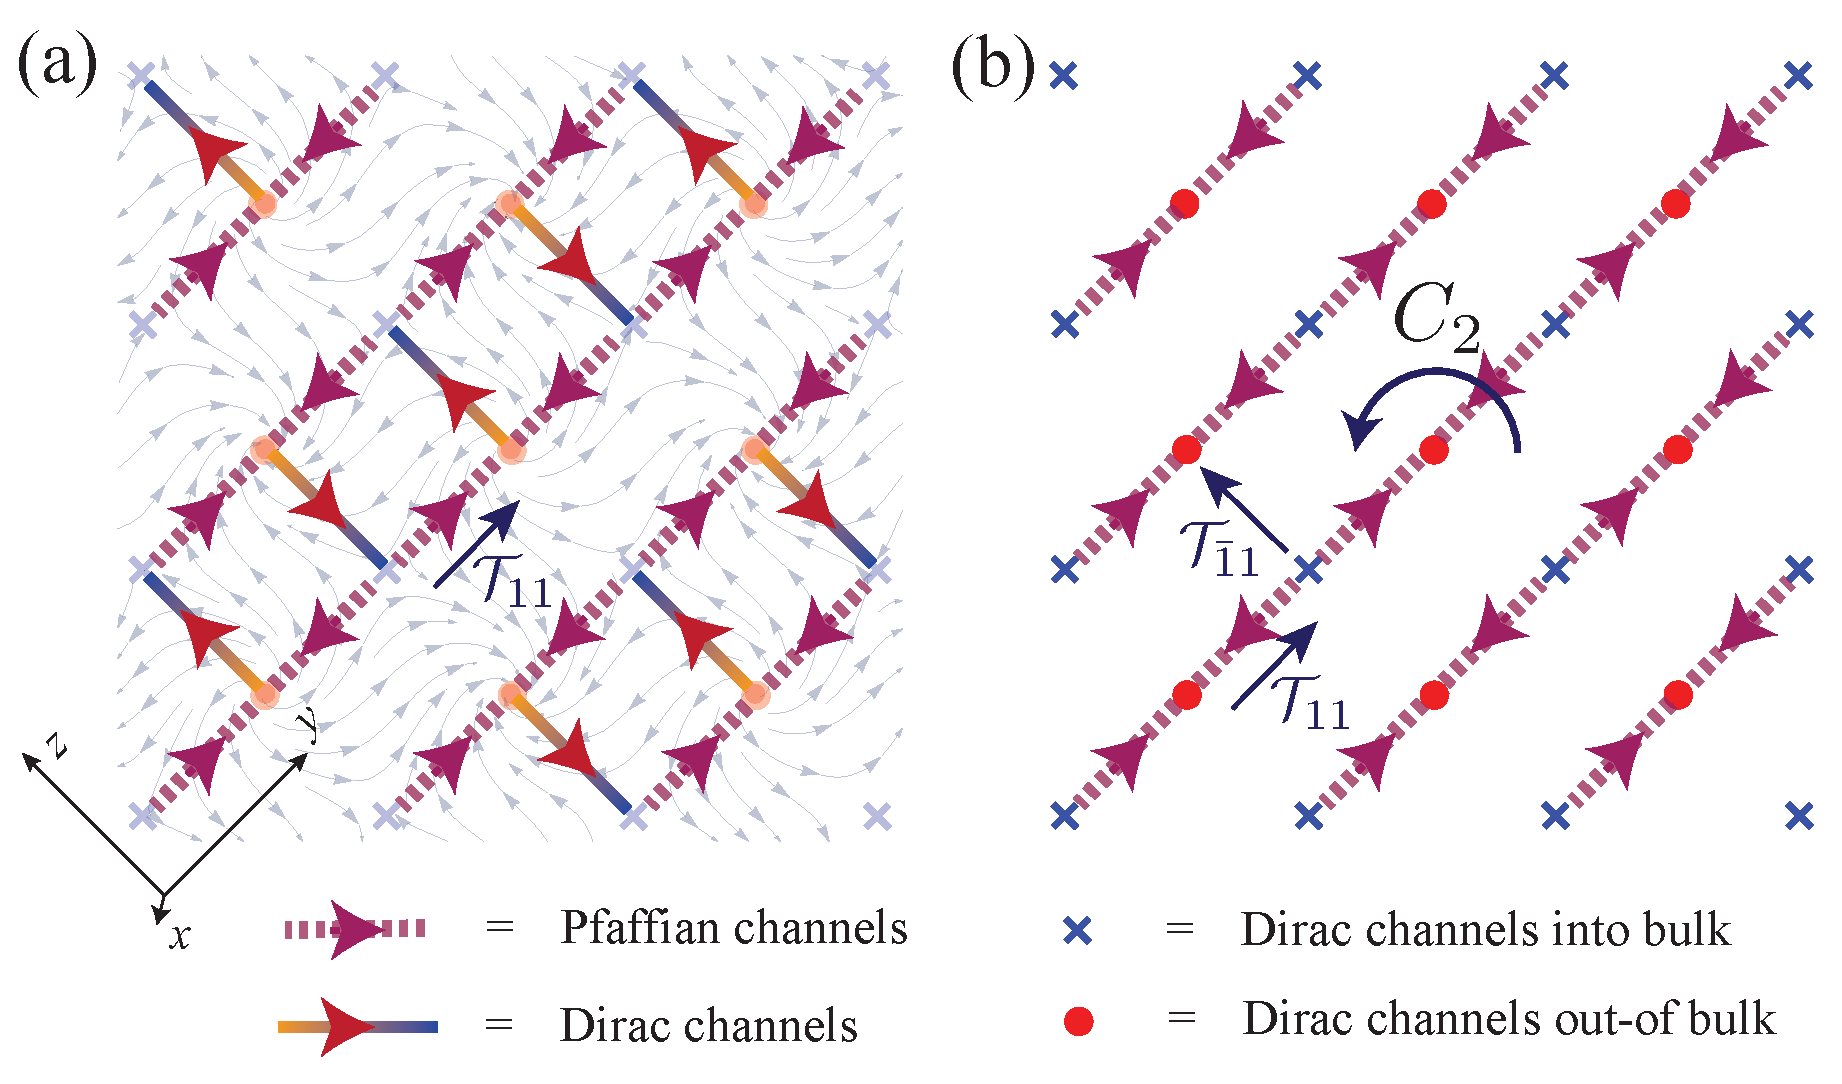
\includegraphics[width=0.48\textwidth]{SurfaceStates}
\caption{Fractional surface states of (a) a 3D Dirac insulator gapped by many-body interaction that preserves $\mathcal{T}_{11}$, and (b) a 3D gapless interaction-enabled Dirac semimetal that preserves $\mathcal{T}_{11}$, $\mathcal{T}_{\bar{1}1}$ and $C_2$.}\label{fig:SurfaceStates}
\end{figure}

First, we consider the coupled wire model with the many-body interaction \eqref{mbdint} (see also figure~\ref{fig:gappinginteraction}) and a boundary surface along the $yz$-plane perpendicular to the wires. The surface network of fractional channels is shown in figure~\ref{fig:SurfaceStates}(a). We assume the bulk chiral Dirac wires ({\color{blue}$\times$}{\color{red}$\bullet$}) are supported as vortices of Dirac mass in the bulk (recall \eqref{DiracHam}), where the texture of the mass parameters is represented by the underlying vector field. The model is juxtaposed along the $yz$- boundary plane against the trivial Dirac insulating state $H_{\mathrm{vacuum}}=\hbar v{\bf k}\cdot\vec{s}\mu_z+m_0\mu_x$, which models the vacuum. The line segments on the surface plane where the Dirac mass $m_0\mu_x$ changes sign host chiral Dirac channels (c.f.~subsection~\ref{sec:fermiarcAFTRpreserving}).

Unlike the single-body (semi)metallic case in figure~\ref{fig:SurfaceStates1bdy} where the surface Dirac channels connects with the bulk ones, now the many-body interacting bulk is insulating and does not carry low-energy gapless excitations. Thus, the surface Dirac channels here cannot leak into the bulk and must dissipate to other low-energy degrees of freedom on the surface. The many-body interwire backscattering interaction in \eqref{mbdint} (and figure~\ref{fig:gappinginteraction}) leaves behind chiral Pfaffian channels on the surface. These fractional channels connect back to the surface Dirac channels in pairs. The surface network of chiral channels preserves the \AFTR $\mathcal{T}_{11}$ symmetry. However, the low-energy surface state is not protected. Electronic states can be localized by dimerizing the Pfaffian channels in the $z$ (or $\bar{1}1$) direction.

Second, we consider the interaction-enabled Dirac semimetallic model summarized in figure~\ref{fig:intenable}(b) in section~\ref{sec:intenable} and again let it terminate along the symmetry preserving $yz$-plane perpendicular to the wires. The surface gapless channels are shown in figure~\ref{fig:SurfaceStates}(b). Here, the semimetallic bulk preserves $C_2$ as well as the two \AFTR symmetries $\mathcal{T}_{11}$ and $\mathcal{T}_{\bar{1}1}$. The bulk array of wires are true $(1+1)$D systems and are not supported as edge modes or vortices of a higher dimensional bulk. The pair of into-paper Dirac modes are bent into the pair of out-of-paper ones along each wire at the terminal. Similar to the previous case, the many-body bulk interwire backscattering interaction leaves behind surface chiral Pfaffian channels. Through the mode bending at the wire terminal, these Pfaffian channels join in pairs and connect to the chiral Dirac channels in the bulk that constitute the Dirac semimetal. In this case, the surface state is protected by $C_2$, $\mathcal{T}_{11}$ and $\mathcal{T}_{\bar{1}1}$, and is forced to carry fractional gapless excitations as a consequence and signature of the anomalous symmetries. For instance, the charge $e/4$ Ising-like quasiparticle and the charge $e/2$ semion can in principle be detected by shot noise tunneling experiments. These gapless fractional excitations however are localized on the surface because the Dirac (semi)metallic bulk only supports gapless electronic quasiparticles.


